%%%%%%%%%%%%%%%%%%%%%%%%%%% asme2ej.tex %%%%%%%%%%%%%%%%%%%%%%%%%%%%%%%
% Template for producing ASME-format journal articles using LaTeX    %
% Written by   Harry H. Cheng, Professor and Director                %
%              Integration Engineering Laboratory                    %
%              Department of Mechanical and Aeronautical Engineering %
%              University of California                              %
%              Davis, CA 95616                                       %
%              Tel: (530) 752-5020 (office)                          %
%                   (530) 752-1028 (lab)                             %
%              Fax: (530) 752-4158                                   %
%              Email: hhcheng@ucdavis.edu                            %
%              WWW:   http://iel.ucdavis.edu/people/cheng.html       %
%              May 7, 1994                                           %
% Modified: February 16, 2001 by Harry H. Cheng                      %
% Modified: January  01, 2003 by Geoffrey R. Shiflett                %
% Use at your own risk, send complaints to /dev/null                 %
%%%%%%%%%%%%%%%%%%%%%%%%%%%%%%%%%%%%%%%%%%%%%%%%%%%%%%%%%%%%%%%%%%%%%%

%%% use twocolumn and 10pt options with the asme2ej format
\documentclass[twocolumn,10pt]{asme2ej}

\usepackage{epsfig} %% for loading postscript figures
\usepackage[ruled]{algorithm2e}
\usepackage{subcaption}



%% The class has several options
%  onecolumn/twocolumn - format for one or two columns per page
%  10pt/11pt/12pt - use 10, 11, or 12 point font
%  oneside/twoside - format for oneside/twosided printing
%  final/draft - format for final/draft copy
%  cleanfoot - take out copyright info in footer leave page number
%  cleanhead - take out the conference banner on the title page
%  titlepage/notitlepage - put in titlepage or leave out titlepage
%  
%% The default is oneside, onecolumn, 10pt, final


\title{Learning Tensegrity Locomotion using Open Loop Control Signals}

%%% first author
\author{Atil Iscen
    \affiliation{
 	Oregon State University\\
	Corvallis, Oregon 97331\\
    iscena@onid.orst.edu
    }	
}

%%% second author
%%% remove the following entry for single author papers
%%% add more entries for additional authors
\author{Ken Caluwaerts
    \affiliation{Reservoir Lab, Ghent University\\
	Ghent, Belgium\\
        ken.caluwaerts@ugent.be
    }
}

%%% third author
%%% remove the following entry for single author papers
%%% add more entries for additional authors
\author{Jonathan Bruce\\
        USRA/University of California Santa Cruz, CA 95064, USA\\
        jbruce@soe.ucsc.edu\\
       {\tensfb Adrian Agogino}
    \affiliation{UC Santa Cruz / NASA Ames Research Center, MS 269-3, Moffett Field, CA 94035, USA\\
        adrian.k.agogino@nasa.gov\\
		}
		{\tensfb Vytas SunSpiral}
    \affiliation{SGT Inc. / NASA Ames Research Center, MS 269-3, Moffett Field, CA 94035, USA\\
		vytas.sunspiral@nasa.gov\\
		}
		{\tensfb Kagan Tumer}
    \affiliation{Oregon State University, Corvallis, OR, 97331, USA\\
		kagan.tumer@oregonstate.edu}
}


\begin{document}

\maketitle    

%%%%%%%%%%%%%%%%%%%%%%%%%%%%%%%%%%%%%%%%%%%%%%%%%%%%%%%%%%%%%%%%%%%%%%
\begin{abstract}
{\it Tensegrity structures offer many advantages to mobile robots while also presenting challenges that include highly non-linear interactions and oscillatory dynamics. These challenges make tensegrity robots hard to control using classical control methods. We take the model of SUPERBall, an icosahedron tensegrity robot that is under production at NASA Ames Research Center, and study the rolling locomotion using an accurate model of the SUPERBall simulated in NASA Tensegrity Robotics Toolkit. We use a distributed and learning based controls approach using coevolutionary algorithms and different types of open loop control signals. Being simple and distributed, these controllers can be readily implemented on the SUPERBall hardware without requiring sensor information and precise coordination. We first analyze  signals of different complexities and frequencies. The results show that with the right types of signals and evolutionary algorithms, the robot can learn rolling locomotion. Among the learned policies, we take one of the best ones to analyze further. We make sure that the resulting behavior is within the capabilities of the hardware by looking at different aspects of the rolling gait such as lengths, tensions and energy consumption. We also discuss the correlation between different signals controlling different parts of the tensegrity robot.
}
\end{abstract}

%%%%%%%%%%%%%%%%%%%%%%%%%%%%%%%%%%%%%%%%%%%%%%%%%%%%%%%%%%%%%%%%%%%%%

%\begin{nomenclature}
%TODO: learn what nomenclature is. Next, delete this section.
%
%\entry{A}{You may include nomenclature here.}
%\entry{$\alpha$}{There are two arguments for each entry of the nomemclature environment, the symbol and the definition.}
%\end{nomenclature}

%%%%%%%%%%%%%%%%%%%%%%%%%%%%%%%%%%%%%%%%%%%%%%%%%%%%%%%%%%%%%%%%%%%%%%

\section{Introduction}
\label{sec:Intro}

Tensegrity robots are part of an exciting emerging field of soft-body robotics that brings many challenges from the controls perspective due to the nonlinear interactions between different elements. Fortunately, learning based controls combined with the distributed nature of tensegrity robots can provide a simplified controls solution to the fairly complex problem of locomotion of tensegrity robots.


 \begin{figure}[t]
   \centering
   \includegraphics[width=\columnwidth]{fig/tensegrity.eps} 
   \caption{An icosahedron tensegrity structure composed of 6 compression and 24 tension elements.}
   \label{fig:basic_diagram}
\end{figure}

Tensegrity structures are based on a simple principle:  the structure is composed of pure tension and pure compression elements. Axially loaded compression elements are encompassed within a network of tensional elements, and thus each element experiences either pure compression or pure tension.  Based on this simple principle, the structures can be arbitrarily complex and stiff by increasing the number of members and by changing their stiffness.



Since the structure does not have any bending or shear forces that must be resisted, individual elements can be extremely lightweight. Moreover, the structure is mostly composed of tension elements that are significantly lighter than the compression elements.  A unique property of tensegrity structures is how they can internally distribute forces.  As there are no lever arms, forces do not magnify into joints or other common points of failure.  Rather, externally applied forces distribute through the structure via multiple load paths, creating a system level robustness and tolerance to forces applied from any direction.  Thus tensegrity structures can be easily reoriented and are ideally suited for operation in dynamic environments where contact forces cannot always be predicted.

 
Tensegrities have a number of beneficial properties including:
\begin{itemize}
\item {\bf Lightweight}: Forces align axially with components and shocks distribute through the tensegrity, allowing tensegrities to be made of lightweight tubes/rods and cables/elastic lines.
\item {\bf Energy efficient}: Through the use of elastic tensile components and dynamic gaits, efficient movement is possible.
\item {\bf Robust to failures}: Tensegrities are naturally distributed systems and can gracefully degrade performance in the event of actuation or structural failure.
\item {\bf Capable of unique modes of locomotion}: Tensegrities can roll, crawl, gallop, swim or flap wings depending on construction and need.
\item {\bf Impact tolerant and compliant}: Since forces are distributed upon impact, they can fall or bump into things at moderate speed. In addition, their compliance ensures that they do minimal damage to objects they contact.
\item {\bf Naturally distributed control}: Characteristics of force propagation in tensegrities allows effective local controllers.
\end{itemize}
The last property is the most subtle but important. In ``traditional'' robots, distributed controls becomes messy due to the need to communicate global state information to all the controllers with high precision, and thus often undermining the very promise of distribution.  Fundamentally, this stems from the fact that a rigidly connected structure will magnify forces internally through leverage, and will accumulate force into joints.  Thus, the actions of a local distributed controller can have disproportionate global consequences. These consequences can require a certain amount of global coordination and state management, undermining the value of the local controller. Tensegrity structures are different, due to the tension network, there is no leverage in the structure.  Thus, forces {\em diffuse} through the structure, rather than accumulate in joints.  As a result, actions by a local controller diffuse through the structure, integrating with all the other local controllers.  While any one local controller will impact the structure globally, that impact is locality relevant and not magnified via leverage. Thus, the structure enables true distributed control, because local actions stay (predominately) local.

Despite these desirable properties, tensegrity robots have remained mostly a novelty for many years due to properties that make them hard to control with traditional control algorithms such as:
\begin{enumerate}
\item {\bf Nonlinear dynamics}: A force generated on one part of the tensegrity propagates in a nonlinear way through the entire tensegrity, causing shape changes, which further change force propagations. 
\item {\bf Complex oscillatory motions}: Tensegrity robots tend to have oscillatory motions influenced by their interactions with their environment.
\end{enumerate}
Fortunately the combinatorial optimization capabilities of learning based controls is a natural match to these problems. Evolutionary algorithms can learn complex control policies that maximize a performance criterion without needing to handle the oscillatory motions and distributed interactions explicitly. Cooperative Coevolutionary Algorithms (CCEAs) enable different controllers that are distributed throughout the tensegrity to learn a cooperative task such as rolling locomotion. The set of the learned policies for these controllers form a unified policy that provides locomotion of the whole robot.

Considering the positive properties of tensegrity robots discussed above, NASA is currently working on using a tensegrity robot for planetary landing and exploration missions as part of the NASA Innovative Advanced Concepts (NIAC) program \cite{NIACfinalreport}. For this program, SUPERBall is a  close to sphere shaped, icosahedron tensegrity robot that is designed and currently under production at NASA Ames Research Center \cite{NIACfinalreport}.  In this work, we use SUPERBall (Spherical Underactuated Planetary Exploration Robot) as our tensegrity robot model. To simulate the robot and learn the rolling locomotion, we use our highly accurate tensegrity simulator NASA Tensegrity Robotics Toolkit (NTRT).

In this work, we combine a simple set controllers and evolutionary algorithms  to obtain rolling locomotion for SUPERBall hardware. Being simple and distributed, these controllers can be readily implemented on the SUPERBall hardware without requiring sensor information and precise coordination. We make sure that the controllers and the rolling behavior is within the limits of the hardware by analyzing the rolling behavior from different perspectives. We also analyze the similarities of the learned signals for different parts of the robot.

The rest of the paper is organized as follows: Section \ref{sec:background} introduces necessary background information and related work. Section \ref{sec:platform} defines the control problem and open loop controls schema that we use. Section \ref{sec:learning} introduces the learning method that we use and presents the results of `learning to roll' for different types of signals. Section \ref{sec:results} analyzes the learned rolling behavior from different perspectives such as movement, energy efficiency and feasibility. Section \ref{sec:signals} analyzes the correlation between the signals that control different parts of the robot while providing the rolling behavior. The paper ends with Section \ref{sec:conclusion}, where we discuss conclusions and  future research directions.

\section{Background and Previous Work}
\label{sec:background}

Tensegrity structures are a fairly modern concept, having been initially explored in the 1960's by Buckminster Fuller \cite{Fuller_Tensegrity} and the artist Kenneth Snelson \cite{Snelson_patent}.  The word tensegrity is formed using the words `tensional integrity'. The structure has an internal balance while the tensile elements encounter constant tension. The early research on tensegrities was first concentrated on the design and analysis of static structures \cite{Skelton2009,BelHadjAli2010a,Juan2008}. The tensegrity principle was used in big structures such as tower or bridges as well as small structures such as toys or furniture \cite{tensegrity_tower}.

The concept of tensegrity is also being discovered in biological systems from individual cells to mamalian physiology \cite{ingber,tensegrity_spine}. Emerging biomechanical theories are shifting foces from bone-centric models to fascia-centric models, where fascia is the connective tissues (muscles, ligaments, tendons, etc.). In the "bio-tensegrity" model, bones are under compression, and continuous network of fascia acts as the primary load path for the body. Inspired by this, since the cables of the robot are the tensional elements that can change length  we use the term `muscle' for the rest of the paper.


Research into control of tensegrity structures was initiated in the mid-1990's, with initial efforts at formalizing the dynamics of tensegrity structures only recently emerging \cite{Skelton2009,motro2003tensegrity,wroldsen2006discussion}. The very properties that make tensegrities ideal for physical interaction with the environment (compliance, multi-path load distribution, nonlinear dynamics, etc.) also present significant challenges to traditional control approaches. 

For the first few decades, the majority of tensegrity related research was concerned with form-finding techniques \cite{Force_Density, Algebraic_form, Review_form_finding,Rieffel:2009:ADO:1507770.1507951, Nonregular_form_finding,Paul:2005:EFT:1068009.1068011,pugh1976introduction}.
The problem of finding the correct configuration to deform a tensegrity robot to a specific shape is already a hard research problem due to the nature of the structure. To solve this problem, there are both algebraic studies as well as evolutionary algorithms. There have also been studies to generate different tensegrity structures using evolutionary algorithms.

In terms of locomotion, tensegrity robots are capable of providing different forms of locomotion due to the diversity of the shapes of the structures \cite{fujiia2006movement}.  Numerous tensegrity locomotion studies use simple irregular tensegrities with 3 or 4 struts \cite{paul2006design,paul2005gait}.  One recent example is a tensegrity snake robot made of nested tetrahedral components which is capable of crawling over a wide range of terrains using a neurologically inspired distributed Central Pattern Generators (CPG's) control network \cite{Tietz2013}.  Here, we are interested in a icosahedron tensegrity robots as shown in Figures \ref{fig:basic_diagram} and \ref{fig:robots} which are made of 6 struts with equal lengths and 24 muscles that connect the end of the struts.

The icosahedron tensegrity provides additional advantages such as rolling locomotion and deployability. The structure is the simplest tensegrity to provide an overall shape close to a sphere. It can handle external forces and impact with the ground easily by deforming. As expected, the impact is diffused through the network of tensional elements. Moreover, the structure is easily collapsible to a star pattern by loosening tensional elements. These properties make icosahedron tensegrity a great option as landing and explotary device for space missions. SunSpiral et al explains the usage of an icosahedron tensegrity robot both as an Entry, Descent and Landing (EDL) instrument and also as an mobility device for a mission to Titan \cite{Vytas_IPPW_2013}. This idea of development and locomotion of an icosahedron tensegrity robot as a space exploration device is part of a project funded by NASA Innovative Advanced Concepts (NIAC) program \cite{NIACfinalreport}.

\begin{figure}[t]
   \centering
   \includegraphics[width=\columnwidth]{fig/robots.eps} 
   \caption{ReCTeR (left), a tensegrity robot and one strut of the modular SUPERBall (right) that is under development at NASA Ames Research Center.}
   \label{fig:robots}
\end{figure}

The literature contains few studies about active control of icosahedron tensegrities. Shibata et al analyzes different surface patterns to roll \cite{shibata2009crawling,shibata2010moving,koizumi2012rolling}. Rieffel at al uses vibration frequencies for locomotion without rolling \cite{morphological_communication}.
Not only icosahedron tensegrities, but also the whole field of active control of tensegrities is still fairly new. A recent review \cite{Dynamics_Review} shows that there are still many open problems in actively controlling tensegrities.

There are few hardware implementations for tensegrity robots. Koizumi et al.\ use a tethered icosahedron robot with pneumatic actuators to analyze base patterns for low energy rolling \cite{koizumi2012rolling}. Rieffel et al.\ uses an icosahedron robot with vibrational motors analyzing forward motion with vibration \cite{morphological_communication}. Suitable for rolling locomotion, ReCTeR is the closest to the ideal icosahedron robot \cite{2917079}. It is untethered, has six motors that control the lengths of six muscles. The robot is composed of a passive shell with 24 muscles. These 24 muscles are essential for the icosahedron. In ReCTeR, these 24 muscles are passive but the structure has 6 additional active muscles that change their length for deformation and locomotion.

SUPERBall is designed in a modular way so that each strut has 2 motors controlling two active muscles, and the struts can be used in different tensegrity robots other than icosahedron. Overall, the next prototype of SUPERBall will have an active outer shell with 12 active and 12 passive muscles, and it will be able to handle strong collisions and torque requirements for rolling locomotion in different types of terrains. In this paper, we analyze the case for 24 active muscles to use the full capabilities of a icosahedron tensegrity, but reducing the number of the controllers is part of our future work.




\subsection{SUPERBall}
SUPERball (Spherical Underactuated Planetary Exploration Robot) is a tensegrity icosahedron robot currently under development at the NASA Ames Research Center  (Figure \ref{fig:SUPERBall}).
%\cite{Caluwaerts2013rsif}.
Its main design goal is to be a more capable robot than a prior prototype called \emph{ReCTeR}, to provide more reliable sensor equipment and  to handle rougher environments.


ReCTeR is underactuated and can roll by actuating six tensile elements running through the center of the robot.
A passive tensegrity icosahedron (24 tensile elements) forms ReCTeR's outer shell, the six actuated members connect opposite sides of the shell.
Hence, only $20\%$ of ReCTeRs tensile members are actuated. 

For SUPERball, the goal is to have the possibility to actuate all tensile elements. The current prototype is going to have 12 actuated tensile elements out of 24, but considering our future goal, this paper studies the fully actuated robot.
The main rationale for full actuation is that we aim to explore various control strategies (e.g. the one presented in this work) without hardware limitations and have precise manipulation capabilities (e.g. for end effector or payload positioning). 



With a total mass of $1.1kg$ (batteries included), ReCTeR cannot carry any scientific payload without a significant impact on the robot dynamics.
This is another reason to develop a new platform. SUPERball's mass with $50\%$ actuated tensile members is around $15kg$.
This larger mass will allow us to explore the behavior of tensegrity robots with a small payload suspended by tensile elements in the center of the robot \cite{Vytas_IPPW_2013}. 
Another important improvement is SUPERball's high power-to-weight ratio. 
ReCTeR's small brushed DC motors are often maxed out ($25W/kg$), while SUPERball has significant headroom ($>80W/kg$, final design $>100W/kg$).
This allows for dynamic motion even in energetically suboptimal regimes.

\begin{figure}[t]
   \centering
   \includegraphics[width=\columnwidth]{fig/strut.eps} 
   \caption{Cross section of the end of the rod for the current design of the SUPERBall.}
   \label{fig:SUPERBall}
\end{figure}


Typical spring tensions are $5N$ to $20N$ for ReCTeR, while the average tension in SUPERball's current configuration is $50N$.
The SUPERball hardware is designed to handle tensile forces up to $500N$.  
One interesting aspect of the tensegrity icosahedron configuration is that the design can conveniently be scaled up or down.
Forces scale approximately linear as a function of the robot's mass. 
For practical purposes, SUPERball is deployed in its minimum diameter configuration (struts of approx. $1.5m$ in length).

Increasing the diameter of the robot does not significantly increase its total mass, because lightweight hollow aluminum tubes are used to connect the end caps.
More precisely, we are using $35mm$ diameter tubes with a $1.25mm$ wall thickness. 
These tubes currently account for $15\%$ of the robot's mass. 
Tripling the robot's diameter ($4.5m$ struts) with the same end caps, would only increase this fraction to $41\%$ (not considering buckling).
This is an advantage over an airbag design, for which the surface area and thus its mass scales quadratically as a function of the diameter.
It can easily be seen that the payload volume scales cubically as a function of the strut length.
This trivially defeats the square-cube law, because the density of the structure drops as one increases the strut length. 

To simplify our designs and to allow us to explore various morphologies, SUPERball is a highly modular platform.
Its basic element is the end cap, each of which is independent.
Every end cap provides actuation, battery power, various sensors and wireless communication.
In the current design, each SUPERball end cap houses a single $100W$ brushless DC motor and approx. $70Wh$ of battery power.
Thus, we can currently control twelve tensile members in the icosahedron configuration ($50\%$).
The sensory equipment of each end cap consists of 2 tensile force transducers, a torque sensor on the motor and a 9 degree of freedom inertial measurement unit.

To make the robot compliant, SUPERball has compression springs inside the tube connecting the end caps.
The tensile elements are cable-spring assemblies. 
Each cable runs between two end caps on different struts. The cable runs from the opposing end cap to the spring end cap, passes through a cable housing assembly inside the spring end cap, and connects to a compression spring located within the spring end cap's tube.
%A cable runs between two end caps, goes into a tube through an end cap and connects to a compression spring.
The opposing end cap of the cable connects to a motor in the case of an actuated tensile member or is simply fixed to the opposing end cap for passive elements.
The motor assembly is a wire spindle that winds or unwinds the cable to change the rest length of the tensile member.

Passive and actuated cable-spring assemblies behave as linear springs with a given (possibly varying) rest length.
This can be implemented in hardware in various ways. 
Active tensile elements are actuated by changing their rest length and we will assume constant velocity motors in this paper. 
While not entirely accurate from a hardware perspective, 
we will show in this work that the required motor power for our controllers is significantly below the motors' power rating, which validates this simplification.

\subsection{NASA Tensegrity Robotics Toolkit (NTRT)}

Simulation of Tensegrity robots is critical for application of intelligent controls. Simulation provides multiple advantages such as being able to train controllers faster than training on actual hardware, or using the simulator to explore design options and hardware requirements. In our paper, we use the (soon to be open-source) NTRT \cite{NTRT-web} simulator that is developed on top of the open source Bullet Physics Engine. Bullet Physics Engine is a discrete timestep, iterative physics simulator that handles collisions and interactions between different types of objects \cite{bullet}.

NTRT simulator relies on Bullet Physics Engine to handle movement and collisions of rigid body objects. On the other hand, to simulate the tensional elements, we needed precise elastic components that we can change their length to simulate active controls of the robot. For this purpose, we implemented our own tensional elements that apply tension according to their stretch. Through the rest of the paper, these elements are called `Muscle'. The name `muscle' is inspired from the biotensegrity studies that describe the bones as compressional elements and the muscles as tensional elements. 

A muscle is attached to two different rigid bodies from specific points. We assume that muscles are abstract elements that apply force to these two rigid bodies according to their tensions. They have basic properties such as rest length (length without stretch) and elasticity coefficient. The tension of a muscle is computed by looking at the current distance between two attachment points and the rest length of the muscle. For simulation purposes, we assume that the muscles have negligeable weight compared to the rest of the structure. Moreover, we also ignore the interactions of the muscles with the rest of the environment. These two assumptions are understandable because the tensional elements stay inside the structure and they do not interact with other objects except extreme deformations. Also, the weight of the physical cables vs the weight of the rest of the robot is extremely low.

The active controls of the muscles are done by changing the rest length of the muscle using a constant speed (motor speed). This is modeled after the motors that pull the elastic cables to increase the tension of a specific elastic component. 

NTRT is previously validated with a physical tensegrity robot (ReCTeR) and precise motion capture. The results showed that the simulator can correctly simulate tensegrity structures with a small margin of error (less than 1 \%) for static structure with active controls and a semi static structure that moves step by step. 
% \cite{Caluwaerts2013rsif}.

\section{Controls Problem}
\label{sec:platform}

Controlling a tensegrity robot brings multiple challenges such as distributed controls, nonlinear interactions between components and handling difficult to model dynamics such as oscillations. For this reason traditional centralized controllers and centralized designs are not a good match for a tensegrity robot. In contrast we present a decidedly distributed approach for controlling a tensegrity robot. On the hardware side, the core of our design is an independently controllable rod containing two independent ``end-cap'' controllers on each side of the rod. This model naturally matches the distributed yet holistic nature of a tensegrity. The controllers act independently of each other but they interact through the system, where changing lengths of one of the muscles affects the whole structure in a non-linear way. This behavior can be seen in Figure
\ref{fig:nonlinear}. When we pull only one of the muscles (muscle 13), all the muscles change their length while some of them get shorter and some of them get longer. 

\begin{figure}[t]
\centering
\includegraphics[width=\columnwidth]{results/actuate1/actuate1.eps}
\caption{Change in length of the muscles when one of them (13th) is pulled to 0.5 meters while other muscles keep the same rest length as before.  Grey bars show original length, red show final length. While the robot is at the exact same orientation, the actual lengths of the muscles change in a non-linear way.  Some of the muscles shorten due to the tension introduced by muscle 13, some of the muscles relax.}
\label{fig:nonlinear}
\end{figure}

To facilitate distributed assembly, the controllers communicate via wifi wireless network. This design allows for simplified construction, and reduces cabling problems that could arise if the tensegrity robot needs to roll through adverse conditions. This design is not only distributed, but modular. For a simple six-bar tensegrity, we can simply assemble six identical rods to form the tensegrity robot. In addition for more complex designs additional rods can be used without changing the design of the rods themselves.

Our next challenge is to control a set of assembled rods into a high-performance tensegrity robot. To do this, we need controls that are able to work in a distributed control environment, and also work when wireless communication may not be high-bandwidth or reliable. To overcome this problem, we use distributed controls and distributed learning, where each controller learns its policy, but the overall behavior requires coordination of these controllers to make the tensegrity robot move. The setup described is a coordination learning problem where we have independent learners working towards a shared goal. The details of the learning distributed controls for this setup is described at the Section \ref{sec:learning}.

An additional control challenge is how to handle the physical hardware limitations of each actuation system. Ideally we would like our controller to be able to simply dictate the actual lengths of each muscle it is responsible for. However, due to the overall tension caused by the rest of the structure, the controllers can only provide the rest length of the muscles.  Since the muscles are flexible, the actual lengths change out of the control of the controller. 

In addition, the hardware limitations also play an important role when tensions get higher. Since all the motors in the robot pull against each other, it is possible to reach tensions that the motors cannot handle. Moreover, since the rest of the structure can potentially overpower any one motor, there  is a chance that a motor is back-driven and forced to feed out some of the cable stored on the spool. To address these limitations, if the muscle is experiencing tensions above the motor limit, and the cable is pulled to its maximum length of 1.1 meters, the simulation is stopped and the policy is considered as not feasible.

To stay within the bounds of the physical hardware, we simulate the motors with high level controllers that has constant speed (0.2 m/s) while the tensions stay within reasonable limits. Indeed, the physical motors on the SUPERBall can pull with 0.5 m/s within the tension range that we are dealing with, but we selected 0.2 m/s in order to leave plenty of hardware headroom and also to lower power consumption. While the motors move with constant velocity, the controllers dictate preferred positions for the motors. Dictating preferred position is exactly same as dictating preferred rest length if the cables do not slip. Every timestep, the motors pull or release their cables with constant speed to get closer to their goal. While staying in reasonable tensions, this setup is feasible on the real robot. The assumption is that there is an intermediate controller layer that regulates the voltage vs torque to provide constant speed rotation.

The overall goal of the controller is to have the tensegrity robot roll smoothly within the limitations of the actuation and communications hardware. To accomplish this, we use a periodic open loop controller with parameters that are set by an evolutionary algorithm (note that we have also performed research on closed loop systems, but due to sensor feedback difficulties and overall increased complexity, we are focusing on open loop controllers in this paper). During rolling locomotion, the robot (and the controllers) will repeat the same motion (one full revolution) over and over. Considering that the rolling locomotion is a repetitive behavior, the signals produced by the controllers will be periodic. The key to making this system work is determining the shape of this periodic signal.

Let's assume that the periodicity of the signal is $t$ and we represent the signal as $F(x)$ , $x$ being time within interval $[0,t]$. There are many possible ways to represent this control function. For instance a natural choice would be a sine wave, or a series of overlapping waves to form more complex control policies. To reduce complexity, in this paper we use an even simpler control model: we break down each control interval into sub-intervals and assign different preferred rest lengths for each sub-interval.  Considering the limited velocity of the motors, the motor will slowly move to reach these selected points during those sub-intervals. The control model is essentially a set of overlapping square waves. As an example, we can divide one period to 2 sub-intervals, where the motor will have a preferred length of $y1$ for the first half of the signal, and $y2$ for the second half of the signal. With the motor moving towards $y1$ and $y2$, the resulting signal will be similar to the Figure \ref{fig:signal}. 


\begin{figure}[t]
\centering
\includegraphics[width=\columnwidth]{fig/signal.eps}
\caption{An example signal with 2 sub-intervals with preferred lengths of y1 and y2 and periodicity t.}
\label{fig:signal}
\end{figure}


To generate a signal, the only parameters needed are number of sub-intervals and rest length values for each sub interval. For the specific example given in Figure \ref{fig:signal}, the number of subintervals is 2 and y1 and y2 are the values of preferred rest lengths for those intervals. The example given in the Figure \ref{fig:signal} is a simple signal, and while number of sub-intervals is low, the complexity of the signals that can be generated is limited. On the other hand, the complexity of the possible signals increases with the number of sub-intervals. Due to this, from now on, we will refer to this parameter as the complexity degree  ($n$) of the signal. Depending on the complexity degree and the values of $y_1,y_2,...y_n$, the shape of the signal can change between typical trapezoid, zigzags, stairs or combination of those. 

To summarize, the complexity of the signal depends on $n$ and each controller has $n$ number of inputs depending on the complexity selected. The rest lengths of the signal follows this signal, and actual lengths of the muscles change according to other muscles and interaction of the robot with the environment. Each controller has a separate signal and it controls only one of the motors. 24 motors controls 24 muscles independently but affecting each other with the common goal of rolling locomotion.



\section{Learning to Roll}
\label{sec:learning}



While the control parameters  to generate the signal are straightforward, the interaction between these signals to reach a rolling behavior is highly complex. As explained before, the  nonlinear and oscilattory nature of the problem makes the tensegrity hard to control with classical control methods. The consequences of specific signal combinations can be simulated, but finding the correct signal parameters for a specific behavior is not possible. In this section we explore how we can use the simulation combined with a fitness evaluation to implement an evolutionary algorithm that can evolve a set of control parameters that leads to the desired behavior.

Evolutionary algorithms are a family of biologically inspired learning methods, where new candidate solutions for a problem are generated, evaluated and eliminated repeatedly \cite{back1997handbook}. Evolutionary algorithms consists of the cycle of  forming new members, assigning fitness and selecting the most fit members. This cycle is called a generation and it is repeated until desired behavior is obtained. 

The problem is episodic, the agents have 60 seconds to test their policies. At the end of each episode these candidates are evaluated according to their performance. In the rolling tensegrity problem, we measure the performance as the distance covered in 60 seconds. Formally, the evaluation is defined as:
\begin{equation}
\label{eq:r}
f = d(y_{0,0},y_{0,1},...,y_{0,n},y_{1,0},...,y_{24,n}) \;,
\end{equation}
where, $y_{i,j}$ is the rest length for the $i$th controller and $j$th subinterval. Depending on the complexity of the signals ($n$) selected, there are $24 * n$ parameters to learn. Note that the decomposition of the distance function $d$ is not readily obtainable in closed form. Instead it must be computed from observing simulations or measured from a physical implementation. Also note that our evaluation does not explicitly take any behavior into account besides the distance moved (final position - initial position). Tensegrities can exhibit many different gaits, ranging from hopping to rolling, and many different paths, ranging from spirals to straight lines. However, tensegrities that maximize final vs initial position tend to roll towards one direction. Deviations from this pattern tend to hurt performance.


\begin{algorithm}
 \SetAlgoLined
 \KwData{Population of $n$ elements for each agent}
 \For{i=1..$k$}{
  $random team \leftarrow \emptyset$ \;
  \ForAll{Populations} 
  {
  	$random_team \leftarrow random_agent$\;
  }
  score = evaluate($random_team$) \;
  \ForAll { agents $\in$ $random_team$}
  {
  	agent.history $\leftarrow$ score \;
%  	\If{score $>$ agent.score}
%  	{
%  		agent.score $=$ score \;
%  	}
  }
  }
 \ForAll{ Populations }
 {
   \ForAll { agents}
   {
   	   agent.fitness = average(agent.history) \;
   }
 	order population according to the fitness\;
 	eliminate the last $z$ members\;
 	copy the first $z$ to the last $z$\;
 	mutate the last $z$\;
 	clear history for the last $z$\;
 }
 
\caption{Cooperative coevolutionary Algorithm with Historical Average}
\label{Alg:CCEA-AA}
\end{algorithm}

The problem that we are working on is distributed by nature. The controllers are independent and there is not a centralized mechanism. To work on such problems, cooperative coevolutionary algorithms (CCEA) is a class of algorithms that extends evolutionary algorithms. Instead of one particular solution for the problem, there are multiple agents. Multiple agents have to coordinate to solve a problem or to optimize an outcome \cite{wiegand2003analysis}. Each agent has a separate population that evolves independently. On the other hand, to evaluate the members of these separate populations, the agents have to form a team for fitness assignment, because the task needs cooperation of the agents to maximize the rolling behavior. At each experiment 1 member from each population are chosen randomly to form a team. This set of policies form the team for that experiment. In our problem, we have 24 agents which means 24 populations.

Each agent optimizes $n$ parameters while they are judged based on their performances within different teams formed during evaluation phase. At each evaluation phase, each member is evaluated multiple times. To move on to the elimination phase, each member has to be assigned a single fitness number using these values. The literature contains multiple approaches to this problem such as taking the maximum score (leniency), testing each member with best team so far (hall of fame) or average score \cite{wiegand2003analysis,panait2008theoretical,Iscen:2013aa}.

For this study, we used the historical average method that we previously developed and tested with earlier versions of NTRT to obtain rolling behavior using sine wave signals (REF). In historical average, each member receives its fitness according to the average of their performances, moreover, if a member survives for the next generation (is not eliminated or mutated) the member keeps  its previous experiences. At each generation, the fitness assignment is the average of this growing history of past evaluations. The overall cooperative coevolutionary algorithm with historical average fitness assignment can be found in Algorithm \ref{Alg:CCEA-AA}.



First, we show an example learning session using signals with complexity ($n$) of 5 and period ($t$) of 4 seconds.  Figure \ref{fig:learning} illustrates the distance rolled by the robots over the course of learning. Starting with 0 meters, the robots converge to rolling over 32 meters in 60 seconds. This result shows that successful learning of rolling locomotion using CCEA is possible. In Section \ref{sec:platform} we discussed when a policy is labeled as unfeasible during learning.  The second line at the same Figure (Figure \ref{fig:learning}) shows the rate of unfeasible policies that are tried while learning to roll. While converging to rolling locomotion, unfeasible policies drop to 0. This shows that the learned policy lies within reasonable lengths and tensions, moreover it is also far from the limits since small mutations that are tried during evolution are also feasible.

\begin{figure}[t]
\centering
\includegraphics[width=\columnwidth]{results/failures/learningVsFailures.eps}
\caption{The performance of the robots during the learning session for signals of complexity 5 and period of 4 seconds. As a side result, the percentage of the policies that were failed to stay in reasonable limits are shown with the second line. }
\label{fig:learning}
\end{figure}

Considering that the robot has a shape that is similar to a sphere with a diameter of 1.5 meters, rolling 32 meters  means  approximately 7 revolutions in a minute. This results in 8 seconds per revolution. Considering that we selected 4 seconds as periodicity of the signal, the learned signals  provide half revolution, and applying same signals also results in the other half of the one complete revolution.  This supports the reasoning behind selecting periodic signals to obtain rolling locomotion as a periodic movement of the robot.

\begin{figure}[t]
\centering
\includegraphics[width=\columnwidth]{results/period/period.eps}
\caption{The performance of the converged policies after learning for signals with periods of different lengths, while the complexity is fixed to 5 points. The best performance is reached with signals that are repeated every 4 seconds. Signals with longer periods have a decreasing performance proportional to the inverse of the periodicity.}
\label{fig:period}
\end{figure}


\begin{figure}[t]
\centering
\includegraphics[width=\columnwidth]{results/complexity/complexity.eps}
\caption{The performance of the converged policies after learning for signals with different complexity levels, while the periodicity is fixed to 4 seconds. The best performance is reached with signals that use 5 points. Less complex signals cannot generate rolling locomotion, and more complex signals are hard to learn.}
\label{fig:complexity}
\end{figure}

The first set of experiments illustrated when $n$ and $t$ are selected as 5 and 4 (4 seconds with complexity of 5). Next, we investigate the results of learning using signals with different complexity and periodicity. Figure \ref{fig:period} shows the converged behaviors when we fix  $n$ to 5 and learn using variable $t$. Note that the signal used for different values of $t$ is not the same. The signals are learned from scratch for each value of $t$. 

Clearly, the peak is when the signals have periods of 4 seconds (frequency of 0.25 Hz). When we shorten the period below 4 seconds, the robot cannot learn to roll. One can think that providing the same signal with a higher frequency can provide the same rolling behavior, but when the tensegrity deforms to start rolling with a higher speed, the contact forces from the ground and the reaction of the structure changes completely. When we increase the periodicity to longer than 4 seconds, the frequency drops and the performance gradually decreases as expected. Moreover,  the rolled distance is linearly proportional to the frequency. For the values of $4$ to $8$ seconds, the performance divided by the frequency give the same value ($\frac{33}{1/4} \simeq \frac{27}{1/5} \simeq \frac{22.5}{1/6} \simeq \frac{19}{1/7} \simeq 132 $). 


Next, we investigate the effects of different signal complexity level to the learning.  The period is fixed at 4 seconds, because it gave the best score combined with the complexity of 5 in previous set of experiments (Figure \ref{fig:period}). We started with the complexity of 2, where the signal is simplest possible. It alters between one high value for the first 2 seconds, and one low value for the last 2 seconds. We increase the complexity up to 9 points. The result is illustrated at Figure \ref{fig:complexity}.  The first conclusion is that signals with complexity 2 cannot succeed at learning to roll, but the performance increases with higher complexity. Clearly the controllers need more complex signals to provide rolling locomotion. The peak performance is reached at complexity 5, where the preferred length alters between 5 different points during 5 intervals of 0.8 seconds each. 

The second conclusion of this experiment is seen when the complexity increases even further.  The learned behavior gradually decreases and error bars show that statistical significance goes down. The reason behind this behavior is that the parameters to learn increase linearly, and the problem to learn becomes linearly harder for each controller. Since all the controllers learn simultaneously while interacting with each other, overall hardness of the problem is increased even further. The error bars show that in more complex problems, some statistical tests reach good results while some of them fail completely due to the hardness of the problem.

\section{Analyzing the Rolling Behavior}
\label{sec:results}

In previous section, we showed that learning to roll for a tensegrity robot succeeds with signals of right periodicity and complexity. In this section, we look at the learned behavior and analyze 
the feasibility of the behavior, lengths and tensions during rolling, converged signals and robustness of the behavior.

As a sample learning behavior, we select one of the learned behaviors with periods of 4 seconds and complexity of 5. The learning process for this behavior was illustrated in Section \ref{sec:learning} and Figure \ref{fig:learning}. For each simulation, the robot tests different policies for 60 seconds, and the distance moved is marked as the score. The policies that are tested are updated according to the Cooperative Coevolutionary Algorithm with Historical Average (Algorithm \ref{Alg:CCEA-AA}). For this particular experiment, the robots reach the performance of rolling 32 meters around 5000 simulation steps. As a side result, the percentage of failed policies (due to high tension) reaches 0.

\begin{figure}[t]
\centering
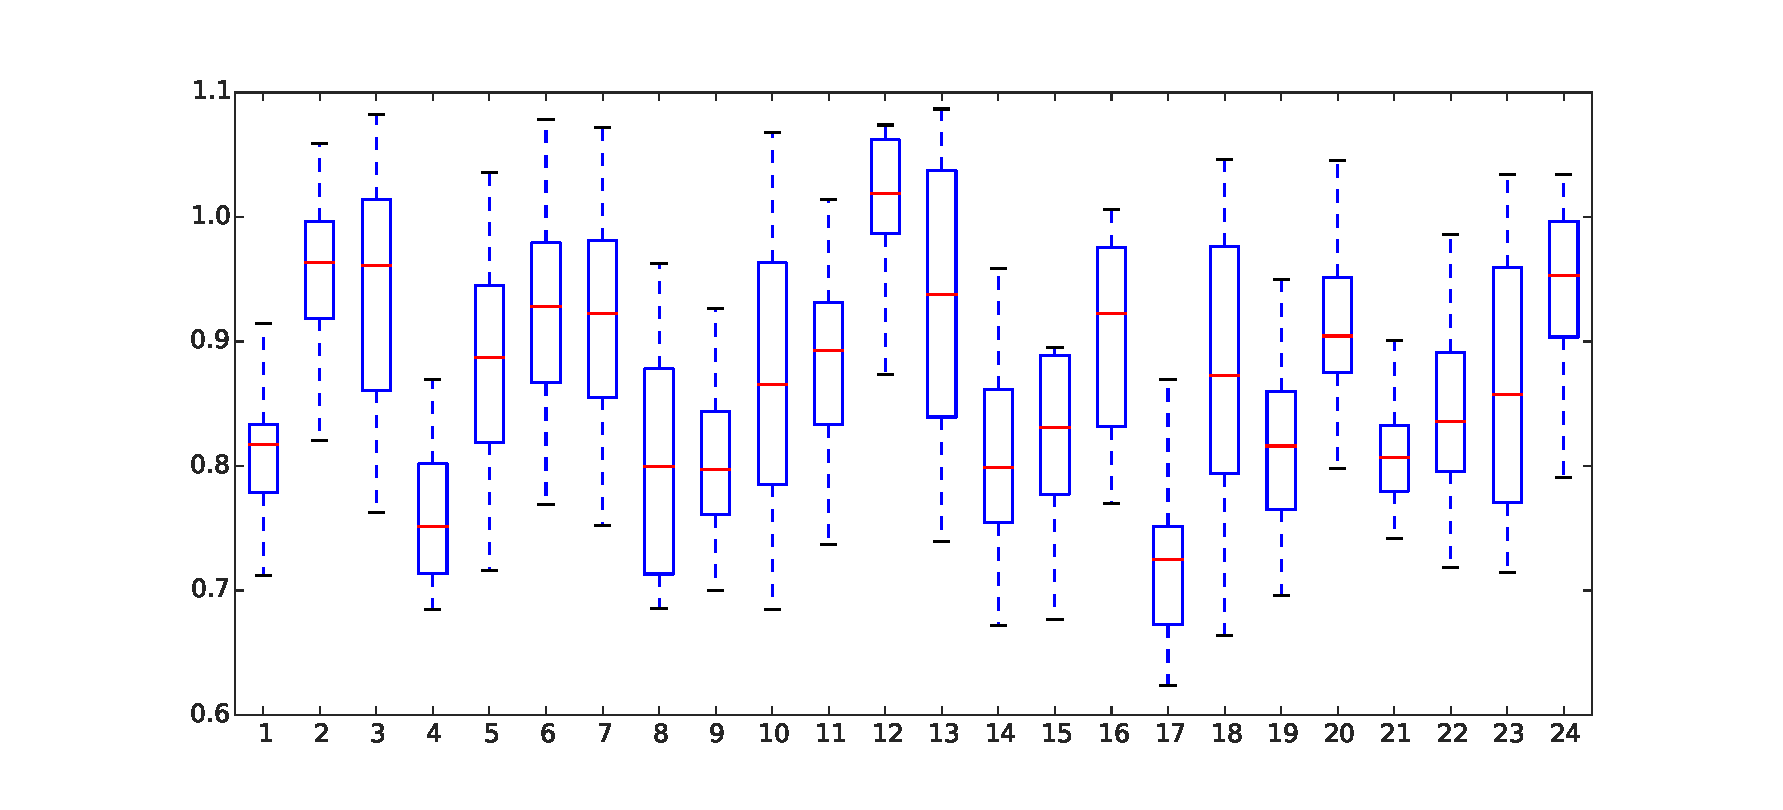
\includegraphics[width=\columnwidth]{results/signals/policy.eps}
\caption{A sample learned policy for 24 motors is illustrated. For each signal, the red line at the center shows the mean of the signal and the box and the dashed lines show the interval that the signal lies in.}
\label{fig:policy}
\end{figure}

First, we take this learned behavior and look at the learned policy. Figure \ref{fig:policy} shows the intervals that each muscle's length lies within.  The muscles' lengths vary from 0.7 m to 1.1 m. While some of the muscles such as 1 and 21 have minimal change in length, some of them (such as 13 and 23) changes bigger intervals. Another remark is that, the mean of the signal (that is noted by the red horizontal line) is not necessarily at the center of the interval that the signal lies in. This is one difference that more complex signals provide. For example, the length of the muscle number 1 is mostly around 0.82 m, but it reaches as low as 0.7 once in a while.
 
\begin{figure}
        \centering
        \begin{subfigure}[b]{0.9\columnwidth}
                \includegraphics[width=\textwidth]{results/tension-energy/lengths.eps}
                \caption{Average Rest Lengths and Actual Lengths of The Muscles}
				\label{fig:lengths}
        \end{subfigure}\\
        \begin{subfigure}[b]{0.9\columnwidth}
				\includegraphics[width=\textwidth]{results/tension-energy/tensions.eps}
                \caption{Average and Maximum Tensions of the Muscles}
				\label{fig:tensions}
        \end{subfigure}\\
        \begin{subfigure}[b]{0.9\columnwidth}
                \includegraphics[width=\textwidth]{results/tension-energy/tensKinEnergy.eps}
                \caption{Kinetic Energy of the Tensegrity Robot}
                \label{fig:KinEnergy}
        \end{subfigure}\\
         \begin{subfigure}[b]{0.9\columnwidth}
         		\includegraphics[width=\textwidth]{results/tension-energy/tensPotEnergy.eps}
                \caption{Total Potential Energy Stored in Muscles}
                \label{fig:PotEnergy}
        \end{subfigure}
        \begin{subfigure}[b]{0.9\columnwidth}
         		\includegraphics[width=\textwidth]{results/tension-energy/power.eps}
                \caption{Power Used by the Motors to Roll}
                \label{fig:power}
        \end{subfigure}
        \caption{Illustration of different aspects of the Tensegrity Robot over time, during rolling locomotion. The used signals for muscles repeat themselves every 4 seconds. The tensegrity robot completes one revolution in 8 seconds. Tensions, Lengths and Power usage of the robot stays in our defined limits for the hardware. }
        \label{fig:RollingAnalyze}
\end{figure}


One way to analyze rolling behavior is looking at the average lengths and tensions of the muscles in addition to the potential and kinetic energy of the structure. First, we look at how the actual lengths of the muscles change compared to the signals provided. Figure \ref{fig:lengths} shows the average rest length of the muscles (signal provided) and the average actual length of the muscles. The area between the two lines shows the stretch of the muscles due to the tension. The most interesting fact about this graph is the difference of frequencies for the two lines. Although the signals that are provided to the muscles repeat themselves every 4 seconds, the actual lengths repeat themselves every 8 seconds. This supports our previous conclusion about using signals that have periodicity of 4 seconds can conclude in revolutions that take 8 seconds. The first half of the roll and second half of the roll use same signal, but the ground interactions make the actual lengths differ.



During the rolling, the average and maximum tensions of the muscles are illustrated in Figure \ref{fig:tensions}. The average tension is low, stays around 60 N. The second line shows the 
the tension of the muscle with longest stretch at each particular time of the simulation. The value goes up to 200N staying in values that our hardware design can handle. The maximum tension graph also repeats itself every 8 seconds as expected.

When we observed  the gait learned using our simulator, we see the rolling locomotion does not have a constant speed. Instead, it slows down and speeds up periodically during each revolution. To illustrate this behavior, we look at the total kinetic energy of all the rods over time in Figure \ref{fig:KinEnergy}. If we take the interval between two peak points (when t=27 and t=35), the kinetic energy stays at zero for 1 second around t=30s. Moreover, the repetitive acceleration and deceleration can be clearly seen. This behavior creates an inefficiency in terms of energy for the gait. There are two main reasons for this behavior: First, the learning algorithm only optimizes the distance rolled, not the energy spent during motion. Optimizing more than one criteria  is actually part of our future work. Second, in this work, we are testing open loop controllers. Using some feedback from the robot (such as lengths, tensions or orientation) having a smoother rolling experience can be possible. This is also another future work that we explain in Section \ref{sec:conclusion}.

Next, we observe the potential energy stored in the muscles. Figure \ref{fig:PotEnergy} shows the pattern that repeats itself every 8 seconds as expected. First 4 seconds and second 4 seconds are similar but they slightly differ due to different environment reaction during the second half of a complete roll. The pattern shows an overall behavior of increasing the potential energy slowly over time, and releasing it. This matches the kinetic energy behavior that we observed in Figure \ref{fig:KinEnergy}. The kinetic energy of the structure increases during the few seconds following the moment potential energy is released (i.e. t=25s).

The last set of experiments analyzes the approximated power usage by the motors during the rolling locomotion. In simulation, the power consumption is approximated using the current tension of the element  and the constant speed that the motors shortens the muscles. As we explained earlier, the learned behavior is not optimized to be power efficient for this study. On the other hand, we want to make sure that it is within limits of motors and batteries that will be used in the hardware. Figure \ref{fig:power} illustrates the average power consumption of the muscles that varies between 2 to 6 W per muscle. Considering that the motors always pull against the tension (and all the muscles are  tight all the time) this value is considerably low. Moreover, it is always possible to lower this value by using a feedback controller in future work.


\section{Analyzing the Roles of Different Muscles}
\label{sec:signals}



\begin{figure}
        \centering
        \begin{subfigure}[b]{\columnwidth}
        		\centering
                \includegraphics[width=0.7\textwidth]{results/signals/aligned1.eps}
                \caption{The signals of the 24 muscles normalized between [$i$,$i$+1] for muscle $i$. After correlation using time offsets, the highest correlated intervals of 4 seconds are  marked with red,yellow,red pattern. }
				\label{fig:aligned1}
        \end{subfigure}\\
         \begin{subfigure}[b]{\columnwidth}
        		\centering
               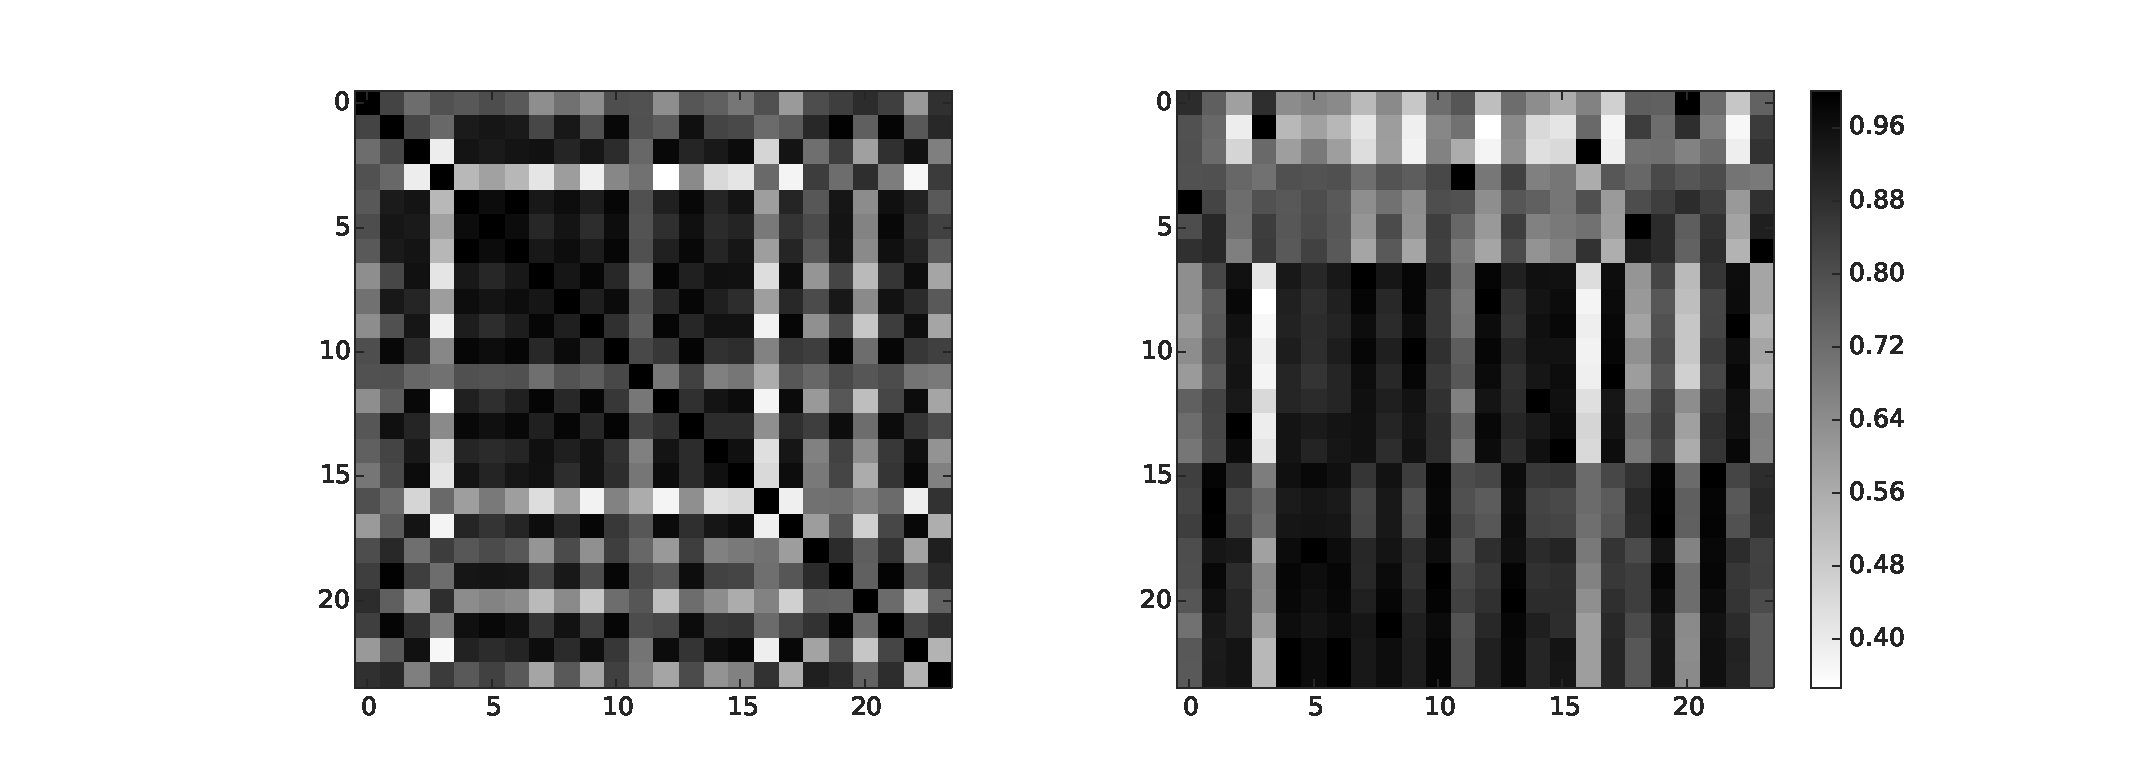
\includegraphics[width=0.7\textwidth]{results/signals/correlation.eps}
                \caption{24x24 Correlation matrix of signals used for each muscle before and after reordering using hierarchical clustering. }
				\label{fig:correlation}
        \end{subfigure}\\
        \begin{subfigure}[b]{\columnwidth}
        		\centering
                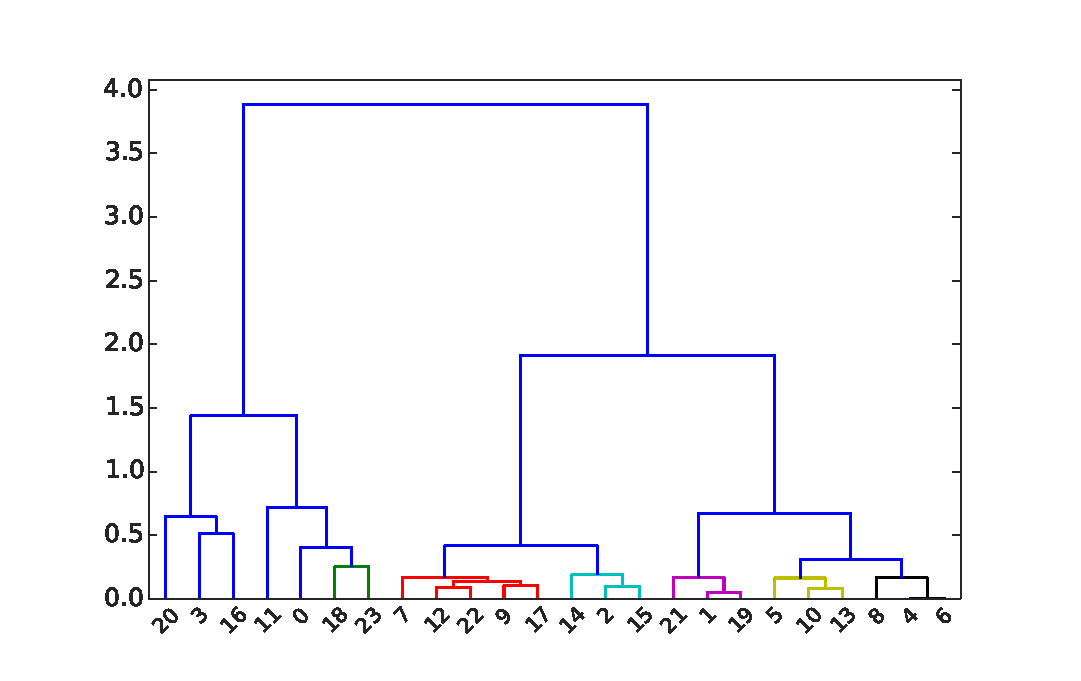
\includegraphics[width=0.7\textwidth]{results/signals/clustering.eps}
                \caption{Result of Hierarchical clustering to cluster and reorder similar signals}
				\label{fig:clustering}
        \end{subfigure}\\
        \begin{subfigure}[b]{\columnwidth}
        		\centering
                \includegraphics[width=0.7\textwidth]{results/signals/aligned2.eps}
                \caption{The signals for the muscles when they are shifted according to the highest correlation and reordered according to the hierarchical clustering. }
				\label{fig:aligned2}
        \end{subfigure}
        \caption{The process of analyzing the signals used for the muscles. The signals are shifted and reordered to show similarities. Subfigure (d) shows that groups of signals have similar patterns.}
        \label{fig:correlationAll}
\end{figure}

Next, we analyze the signals further by looking at their shapes and correlation between them. The top half of the Figure \ref{fig:aligned1} shows all 24 signals when they are normalized between 0 and 1. The purpose of this experiment is to show similarities of signals and different types of signals learned at the end of coevolution. First, we look at the correlation between signals. For each signal, red-yellow-red area highlights the interval that maximizes correlation with other signals. At this ordering, it is hard to see similarities between signals. In Figure \ref{fig:aligned2}, we shift the signals so that their selected intervals match, then we use hierarchical clustering (Figure \ref{fig:clustering}) to group the signals according to the similarity metric. 

After reordering the signals, Figure \ref{fig:aligned2} shows that half of the signals have one peak high and one low, but the other half have 2 signals that are more complex with 2 peak points. This result gives us multiple conclusions. First, the learning algorithm makes use of the complexity provided. Although a subset of the signals is simple, but another subset has more complex signals with  multiple peak points that can only be generated with complexity coefficients that are higher than 3. The subsets of the signals that are similar can be regenerated using different parameters but the same formula. Let's consider a normalized signal as $f(x)$. The formula $g(x)=A+B*f(x+C)$ can produce similar signals for different values of $A$, $B$ and $C$. Using this idea, all 24 signals can be reproduced using 3 to 4 base functions and different parameters. This gives us a hint about why many papers in literature proposes to use central pattern generators to control tensegrity robots. 

The last set of results show how critical each muscle is for a given rolling locomotion. We take the tensegrity robot with the learned policy and disable one of the muscles and observe the effect of such a failure on overall behavior. Figure \ref{fig:disable1} shows that performance depends on which muscle fails. For a significant number of muscles, using the same algorithm still provides rolling behavior with similar performance.  On the other hand some muscles play a critical role for that specific policy.

\begin{figure}[t]
\centering
\includegraphics[width=\columnwidth]{results/testing-disabling1/disabled.eps}
\caption{The performance of the learned policy, when we disable one of the muscles. Learned policy is partially robust to failures of some of the muscles. }
\label{fig:disable1}
\end{figure}

\section{Conclusions and Future Work}
\label{sec:conclusion}

Tensegrity robots have a great potential with their flexibility, deployability, robustness and  different forms of locomotion. Due to these advantages, it is considered as a good candidate for space exploration and mobility missions. On the other hand, controlling a tensegrity robot brings multiple challenges due to the distributed nature and nonlinear interactions between the components. Controlling a tensegrity robot to reach a rolling locomotion is hard to figure out with classical control methods.

In this work, we used coevolutionary algorithms combined with open loop signals to learn distributed rolling locomotion for icosahedron tensegrity robot. We used the model of the robot that is currently under production at NASA Ames Research Center. As a simulator, we used NTRT a simulator for tensegrity robots that closely matches reality. For learning, we analyzed the results of using signals with different complexity levels and different frequencies. The results show that by selecting the right type of signals, learned behavior can reach decent rolling locomotion of 32 meters per minute. 

To study the learned behavior, we used one of the learned policies and analyzed the signals used vs the actual lengths of the muscles, the tensions and energy stored in the structure. The results shows that one complete revolution takes 8 seconds. The muscles use the same signal for the first half of the revolution and second half of the revolution. Moreover the rolling behavior is not smooth, the robot repeatedly accelerates and decelerates during rolling. This causes inefficiency but that is understandable since the learning algorithm does not optimize energy consumption.

Finally, we analyzed the signals of different muscles, and concluded that while some muscles can function with simple signals, others require complex activation patterns. In addition, there is significant similarity and overlap among sets signals, implying interchability fo the muscles. This observation leads us to conclude that in terms of robustness, while some muscles play a critical role for rolling, the presented algorithm can handle failures in some muscle groups. 

In conclusion, we show that the coevolution combined with open loop signals can provide rolling locomotion. Moreover the learned behavior is feasible for the designed hardware that is under production. Currently, there are open research directions for rolling locomotion for tensegrity robots. First, using multi-objective optimization techniques, we are currently investigating minimizing energy consumption and obtaining a smoother rolling behavior. Second, using feedback for the controllers can increase the overall ability of the locomotion. The algorithm can make use of the information about the interaction of the structure. This future research direction can address problems such as rolling on uneven terrains, rolling uphill and rolling when there are external forces to disturb or interrupt the locomotion.


%\section*{Acknowledgment}
%Thanks ... TODO.

\section*{Acknowledgments}
This research was supported by the NASA Innovative Advanced Concepts program.
\mbox{Ken Caluwaerts} was supported by a {Ph.D.} fellowship of the \mbox{Research Foundation - Flanders} (FWO).  Support also came from \mbox{NSF Graduate Research Fellowship} No. DGE1106400, and by NASA Prime Contract Number NAS2-03144 awarded to the University of California, Santa Cruz, University Affiliated Research Center.

The authors would like to thank Andrew P. Sabelhaus, Alice Agogino,  Brian Tietz, Terry Fong and the NASA Ames Intelligent Robotics Group.

\bibliographystyle{asmems4}
\bibliography{references}
\end{document}
